%%%%%%%%%%%%%%%%%%%%%%%%%%%%%%%%%%%%%%%%%
% University/School Laboratory Report
% LaTeX Template
% Version 3.1 (25/3/14)
%
% This template has been downloaded from:
% http://www.LaTeXTemplates.com
%
% Original author:
% Linux and Unix Users Group at Virginia Tech Wiki 
% (https://vtluug.org/wiki/Example_LaTeX_chem_lab_report)
%
% License:
% CC BY-NC-SA 3.0 (http://creativecommons.org/licenses/by-nc-sa/3.0/)
%
%%%%%%%%%%%%%%%%%%%%%%%%%%%%%%%%%%%%%%%%%

%----------------------------------------------------------------------------------------
%	PACKAGES AND DOCUMENT CONFIGURATIONS
%----------------------------------------------------------------------------------------

\documentclass[12pt]{article}

%\usepackage[version=3]{mhchem} % Package for chemical equation typesetting
%\usepackage{siunitx} % Provides the \SI{}{} and \si{} command for typesetting SI units
\usepackage[left=1in,top=1in,right=1in,bottom=1in]{geometry} % Document margins
\usepackage{graphicx} % Required for the inclusion of images
\usepackage{pdfpages}
\usepackage{natbib} % Required to change bibliography style to APA
\usepackage{amsmath} % Required for some math elements 

\setlength\parindent{0pt} % Removes all indentation from paragraphs

\renewcommand{\labelenumi}{\alph{enumi}.} % Make numbering in the enumerate environment by letter rather than number (e.g. section 6)

%\usepackage{times} % Uncomment to use the Times New Roman font

%----------------------------------------------------------------------------------------
%	DOCUMENT INFORMATION
%----------------------------------------------------------------------------------------

\title{\textbf{Find A Room} \\ Sprint 3 Retrospective \\ CS 307} % Title

\author{Team \textsc{13}(Snoxy)} % Author name

\date{\today} % Date for the report

\begin{document}

\maketitle % Insert the title, author and date

\begin{center}
\begin{tabular}{l r}
Members: & Nathan Chang \\ % Partner names
& Xiaojing Ji \\
& Zilun Mai(Owen) \\
& \textbf{Saranyu Phusit(Team Leader)} \\
& Yao Xiao \\
\\
\bigskip
Instructor: & Professor Buster Dunsmore \\% Instructor/supervisor 
Project Coordinator: & Miguel Villarreal-Vasquez % Instructor/supervisor

\end{tabular}
\end{center}

\newpage

% If you wish to include an abstract, uncomment the lines below
% \begin{abstract}
% Abstract text
% \end{abstract}

%----------------------------------------------------------------------------------------
%	SECTION 1
%----------------------------------------------------------------------------------------


\newpage
\section{What went well}

We finished all the tasks.

\textbf{Communication}\\ We decided to work together for the last sprint so that we can have real-time communication among corporate members, and also to help when someone is stuck. \\ \\

\textbf{Presentation}\\ We made a demonstration video to grab people?s attention. We feel like this is the best way of presenting it, and by this way we can also have a precise timing, avoiding potential risks. It turns out in the actual presentation, the video totally met our expectations. We focused highly on features and what the application has to offer rather than showing how it works while presenting. This allowed us to present our application in its entirety.  \\ \\

\textbf{Navigation}\\ The step by step navigation is successful using the BFS algorithm. The route could show up precisely. The generated instruction is clear enough for the user to follow. We also solve the problem when the user stops the navigation midway. \\ \\

\textbf{UI} \\ We improved the entire UI to make it more user friendly.  We provided the UI to ensure everything on the map can be redrew immediately after users re-enter their current location or change their destination during the navigation, so that user can see their update easily. We also provided icons for public facilities quick access and chatting window. More members of the team were working on the UI portion during this sprint, easing the workload for the main UI developer. \\ \\


\section{What didn't go well}

\textbf{Work Spacing}\\
We didn't space all of our work over sprint two's time very well. This lead to very long work sessions and many hours of lost sleep and other days with little to no work being done, because user stories covered on the first two sprints are comparatively easy to be implemented, while the remaining user stories requires a lot of work. \\ \\

\textbf{Framework}\\
We use the cordova framework to generate the mobile app. The framework is agile and easy to use. However, we ran into several problems such as scrolling and positioning, which made us spend a lot of time trying to fix it. \\ \\

\section{What we can improve}
\begin{itemize}
\item \textbf{Start Early} \\ \\
We started to work a bit later than we would have liked and thus we had to overwork on the few days that we did work. 

\item \textbf{Have Work distributed.} \\ \\
We should spend time on distributed work more wisely. For example, some important task which is the pre requirement of other tasks should be done prior to other tasks and should be distributed to best team members.

\end{itemize}

\section{Sprint Details}
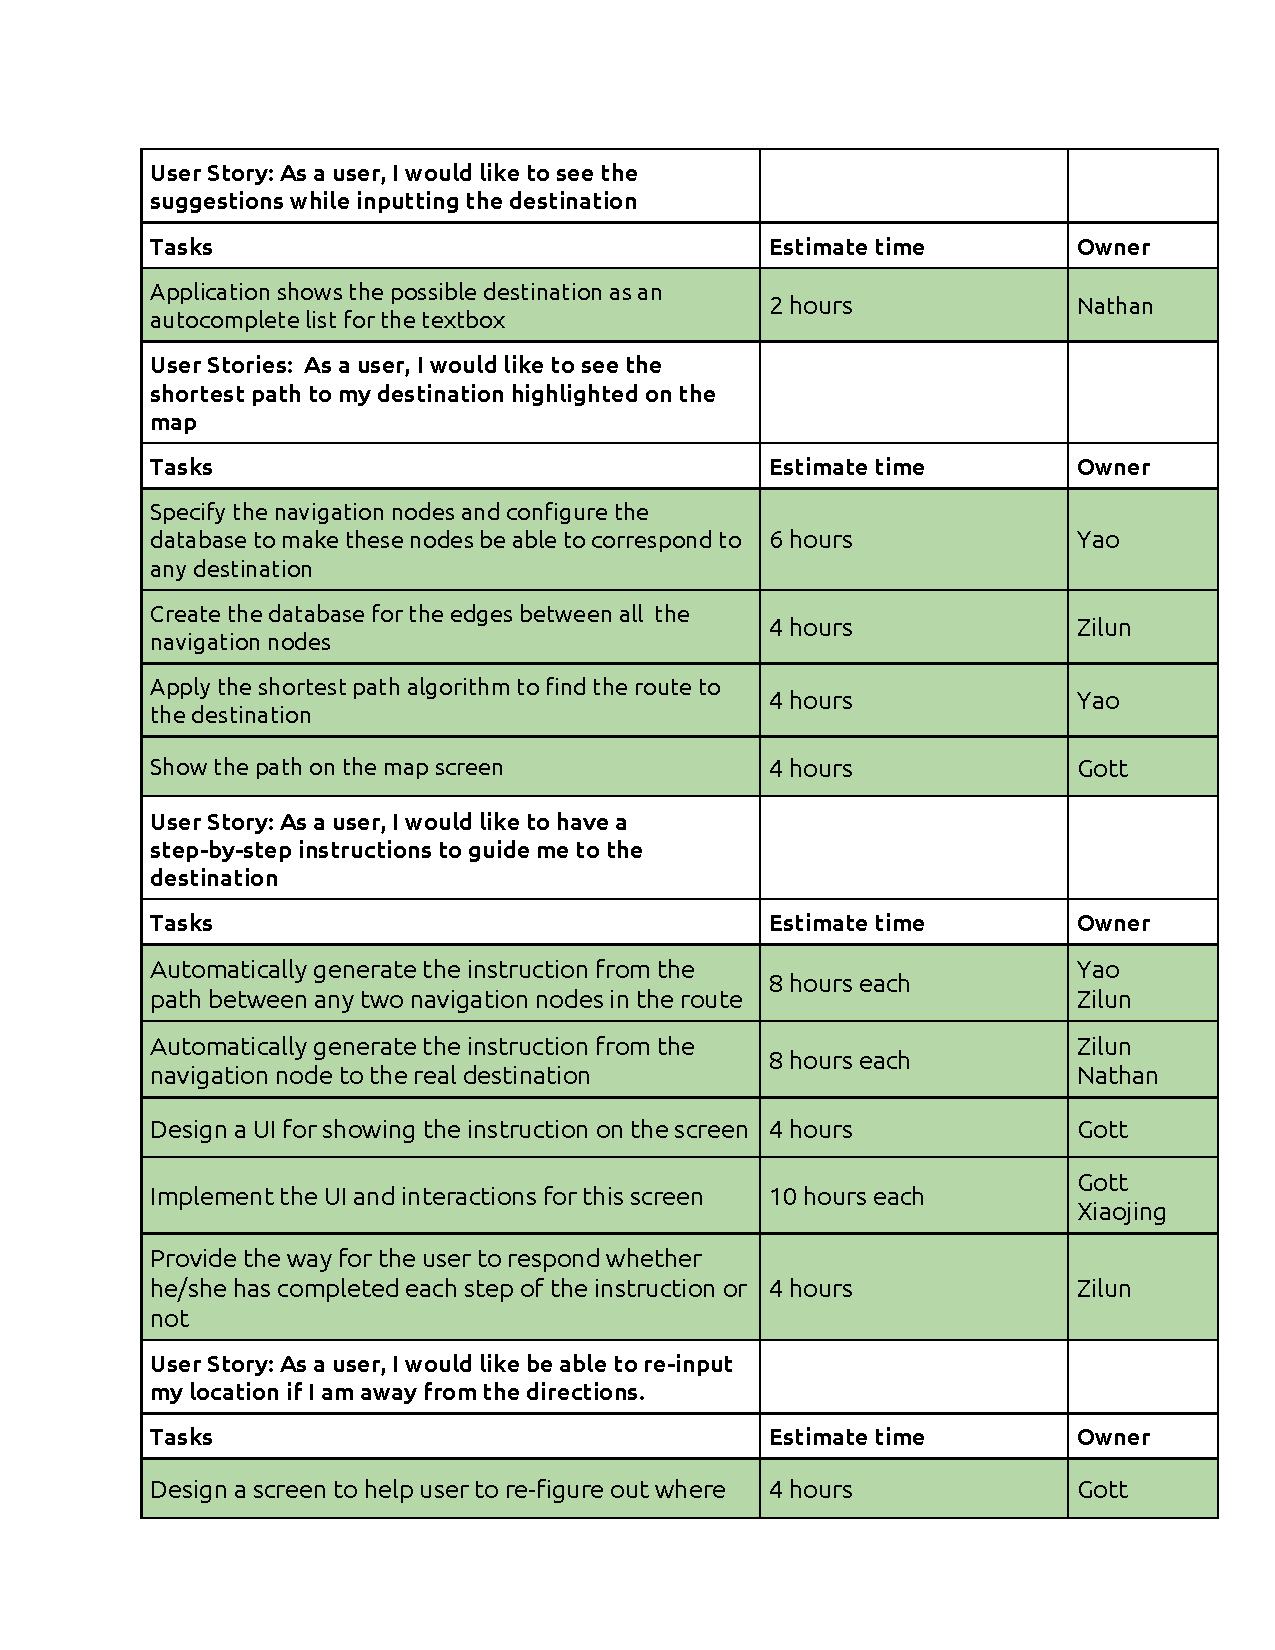
\includepdf[pages={1,2,3}]{task_datails_sprint_3.pdf}

\end{document}